\chapter{On the Resurrection of Jesus}\label{ch:resurrection}
%!TEX root = main.tex

\section{Is the resurrection 97\% likely?}

\subsubsection{The Probability of the Resurrection - Calum Miller \&
Chris Hallquist - Unbelievable? - 06 July 2013 -- Is the resurrection
97\% likely as Swinburne
claims?}\label{theprobabilityoftheresurrection-calummillerchrishallquist-unbelievable-06july2013--istheresurrection97likleyasswinburneclaims}

As part of the
\href{http://brianblais.wordpress.com/2013/02/27/unbelievable-project-a-non-believers-armchair-perspective-on-six-years-of-christian-debates/}{Unbelievable
Project}, I am taking notes and ``arm-chair'' responding to each of the
\href{http://www.premierradio.org.uk/shows/saturday/unbelievable.aspx}{Unbelievable
podcast} episodes satisfying a set of
\href{http://brianblais.wordpress.com/2013/02/27/unbelievable-project-a-non-believers-armchair-perspective-on-six-years-of-christian-debates/}{simple
rules}.

See here for a
\href{http://ondemand.premier.org.uk/unbelievable/AudioFeed.aspx}{full
RSS Feed of the podcasts}.

\paragraph{Description of Episode}\label{descriptionofepisode}

\begin{itemize}
\item
  Full Title: \emph{The Probability of the Resurrection - Calum Miller
  \& Chris Hallquist - Unbelievable? - 06 July 2013 -- Is the
  resurrection 97\% likley as Swinburne claims?}

  \begin{quote}
  Christian philosopher Richard Swinburne has used probability theory to
  show that the likelihood of the resurrection of Christ is 0.97.\\
  Calum Miller is a Christian apologist and student of Swinburne. He
  talks about why he believes that probability theory can be used to
  show that the resurrection is highly likely to be true.\\ Chris
  Hallquist is an atheist blogger who argues that the resurrection is
  not well supported by evidence or probability.\\ For more debates
  visitwww.premier.org.uk/unbelievable\\ Join the conversation
  viaFacebookandTwitter\\ For Calum Miller http://www.dovetheology.com\\
  For Apologetics UK http://apologeticsuk.blogspot.co.uk/\\ For Chris
  Hallquist http://www.patheos.com/blogs/hallq\\ Get the MP3 podcast of
  Unbelievable?http://ondemand.premier.org.uk/unbelievable/AudioFeed.aspxor
  ViaItunes\\ You may also enjoy:\\ Unbelievable? 16th April 2011 -
  Biblical evidence for the Resurrection - Bart Ehrman \& Mike Licona.\\
  Unbelievable? 7 April 2012 - Are the Jesus Scandals evidence for
  Easter? David Instone-Brewer vs Bob Price.
  \end{quote}
\end{itemize}

\href{http://media.premier.org.uk/unbelievable/d8367d64-5f9f-496f-967a-ff4659e83027.mp3}{Download
mp3}.

\begin{itemize}
\itemsep1pt\parskip0pt\parsep0pt
\item
  Justin Brierley - Christian Moderator
\item
  Calum Miller - Christian
\item
  Chris Hallquist - Atheist
\end{itemize}

\paragraph{Notes}\label{notes}

\textbf{Me - I was really looking forward to this episode. What was not
to like? Probability theory, ancient religions, evidence for
Christianity\ldots{}bring it on! Unfortunately, it really wasn't that
impressive.}

Calum - \emph{``There's what's called the confirmation of resurrection,
the explanatory power. And this is basically the idea that there is a
lot of evidence which, if the resurrection happened would be expected
but if the resurrection didn't happen, it would be very improbable. And
if this is true, if there really is that kind of evidence, then it
follows from probability theory that our confidence in the resurrection
should be greatly increased by this evidence. {[}Concerning the
prior{]}, more extraordinary or extreme events are more improbable to
begin with, and so you would need more evidence to confirm them. So a
lot of the debate about the resurrection comes down to the prior
probability, whether we think it is actually really improbable and that
no possible evidence could ever make us convinced of it.''}

\textbf{Me - He basically has the distinction between the following as
the basis for all of the ``calculation'':}

\begin{enumerate}
\def\labelenumi{\arabic{enumi}.}
\itemsep1pt\parskip0pt\parsep0pt
\item
  \textbf{evidence that, if it existed, would be very common if the
  resurrection \emph{did} happen}
\item
  \textbf{evidence that, if it existed, would be very rare if the
  resurrection \emph{didn't} happen}
\item
  \textbf{the prior probability for the resurrection}
\end{enumerate}

**where he admits that *``the debate about the resurrection comes down
to the prior probability*``. Anyone doing probabilistic inference knows
that it should never come down primarily to your choice of priors. The
data needs to rise above the prior, and the prior needs to be an honest
-ideally objective- assessment of the pre-data probability assignments
or, often, the initial state of ignorance. By admitting this, Calum is
essentially saying either that:**

\begin{enumerate}
\def\labelenumi{\arabic{enumi}.}
\itemsep1pt\parskip0pt\parsep0pt
\item
  \textbf{the data are not strong enough to constrain a diffuse prior,
  and thus is unconvincing or\ldots{}}
\item
  \textbf{you have to come into the debate with a \emph{sharp} prior
  which admits to a presupposition of the strength of the claim.}.
\end{enumerate}

\textbf{Neither of these stances is convincing in the slightest.}

\textbf{Further, in response to this set up, he ignores the most
important thing in any Bayesian treatment is the set of models that you
are using to compare. You cannot simply test the truth of a single model
in isolation, nor is it generally informative to compare model A true or
false. Instead one wants to set up a list of models, hypotheses,
theories to explain the data and evaluate those multiple models. Instead
of,}

\$latex\\P(\{\textbackslash{}rm
resurrection\}\textbar{}\{\textbackslash{}rm
data\})\\\$\\and\\\$latex\\P(\textbackslash{}mbox\{not
resurrection\}\textbar{}\{\textbackslash{}rm data\})\\\$

\textbf{you'd want}

\$latex\\P(\{\textbackslash{}rm
resurrection\}\textbar{}\{\textbackslash{}rm data\}),
P(\{\textbackslash{}rm hallucination\}\textbar{}\{\textbackslash{}rm
data\}), P(\{\textbackslash{}rm legend\}\textbar{}\{\textbackslash{}rm
data\}), P(\{\textbackslash{}rm literary\}\textbar{}\{\textbackslash{}rm
data\}), P(\{\textbackslash{}rm hoax\}\textbar{}\{\textbackslash{}rm
data\}),\$ etc\ldots{}\\\textbf{where of course each of these models
would have many details beyond the simple label I'm putting in here. By
being explicit with what you're comparing to, it is easier to see where
the different prior probabilities come in. Are you really going to
suggest that someone rising from the dead is on par, prior to the data,
with a legendary construction given how many legendary constructions
we've seen and how many dead rising we've \emph{not} seen?}

\textbf{What is clear is that all of these other models must, a priori,
be more probable than rising from the dead \emph{even if a God exists}.
Just because you believe miracles \emph{could} happen does not mean that
you believe every miracle claim is true, and given the number of clearly
false miracle claims, the prior probability for any miracle claim must
be quite low - even if you believe miracles actually occur.}

\textbf{Another point about the data which Calum never deals with is
that it should include things we \emph{don't} see, not just things we
do. If we expect something to occur with a claim, and we don't see it,
that is in fact evidence against the claim.}

Chris - Most Christians might discount the claim that the miracles
around African religions seem to disappear in the US and UK because of
lack of faith. Or perhaps the miracle stories around Mormonism. What
makes the miracles of Jesus different than these ones? Once you accept
the idea that resurrection claims can exist quite commonly in a group of
religiously charged people, it is no longer quite so hard to understand
the resurrection claims in the Bible.

Calum - The reports of an empty tomb are exactly what you'd expect if
the resurrection actually happened, and would be unlikely in the case of
a non-resurrection event.

\textbf{Me - Dealing with this is actually very simple. He is correct
that \emph{if the resurrection occurred}, then the report of an empty
tomb would very likely be given, and I would add that it would also be
very likely to be reported in the earliest accounts we have of the
resurrection. Is this what we see? No! The empty tomb is not mentioned
in Paul, neither are the physical visitations, both of which you'd
expect to see if the Resurrection actually occurred. Even the
visitations are not mentioned in Mark! So, from a probabilistic point of
view, this is the exact opposite of what we'd expect to see if the
resurrection actually occurred. In fact the descriptions of the
resurrection get more elaborate and more physical the later the text
(Paul has visions, Mark has no visitations but the empty tomb, Matthew
and Luke have visitations, John has the doubting Thomas story,
etc\ldots{}). This is exactly what we'd expect for legendary
development, or a story that has been embellished over time.}

\textbf{The other thing, is it really all that unlikely to have an empty
tomb story with no resurrection? Notice, I'm not saying to have an empty
tomb, but to have an empty tomb \emph{story}. There are several
different routes to get that. One is as a literary device. I believe
Richard Carrier supports this, as a reference to Daniel. Another is a
deliberate counter to
\href{http://en.wikipedia.org/wiki/Docetism}{Docetism}, to gain favor
and win an argument.}

Calum - \emph{``It is not necessarily helpful to have just some kind of
religious context, it must be the right kind of one. So, for example, I
can see very good reasons why God would want to vindicate Jesus'
teaching by resurrecting him because I think Jesus taught a lot of very
good things, I thought he was (obviously as a Christian) I think he was
a very sincere, a very good person. And I can think of a lot of good
reasons why God would choose Jesus to be a prophet and to become
incarnate in him. Whereas I don't see comparably good reasons why God
would want to vindicate Mormon teaching. Obviously a lot of that is
because I don't know a lot about Mormonism but there's still the
asymmetry there.''}

Chris - The positive evidence for Mormonism is a lot better than for
Christianity. We have signed documents by the early followers and
founders attesting to the miracles. The best we can say about Paul's
evidence is that he had a vision. We have a lot of negative evidence for
Mormonism, to be sure, but if we knew more about Christianity perhaps
things would be different.

\textbf{Me - I would add that we have this \emph{pro-Christian} filter
for all of our documents, a filter called the Middle Ages, where
documents supporting Christianity had a much better probability of
surviving (i.e.~copied) than ones critical of Christianity. The only
reason we have the Nag Hammadi texts is that the monks refused to burn
them, as ordered by the Christian orthodoxy at the time, and instead
chose to store them in a cave. Think about that campaign of whitewashing
for hundreds of years! Actually, the fact that we have so little actual
documentary support for Christianity coming from the first century,
despite this huge bias, to me argues against Christianity.}

Chris- How do you know Jesus was sincere or not? Seems like the same
could be said for Joseph Smith.

\subsubsection{Afterward - a bit about
priors}\label{afterward-abitaboutpriors}

(this section is all \textbf{Me -}, so I won't put it in bold.)

I don't really think that when Calum is referring to priors that he
really means that in the same way as \emph{before the data}. It seems to
me, and I believe Swinburne's analysis reflects this, that the prior for
\emph{this} calculation is really the posterior for a \emph{previous}
calculation regarding the existence and properties of God. This is
perfectly legitimate Bayesian procedure, but it makes the argument a
different one. Because of this,
\href{http://ndpr.nd.edu/news/23553-the-resurrection-of-god-incarnate/}{Swinburne's
calculation} for the probability of God needs to be addressed before we
can even deal with the priors in this resurrection argument. That will
have to be another post entirely, but at any rate Calum did not do it a
service in this debate, having not really gotten to the meat of it when
he could have.



\section{Resurrection and Regression}

Dan Barker has written an Easter Challenge\cite{Barker:1992aa} for
any Christian to come up with a seamless account of what happened on the
day of the Resurrection.

\pquote{The conditions of the challenge are simple and reasonable. In each of
the four Gospels, begin at Easter morning and read to the end of the
book: Matthew 28, Mark 16, Luke 24, and John 20-21. Also read Acts
1:3-12 and Paul's tiny version of the story in I Corinthians 15:3-8.
These 165 verses can be read in a few moments. Then, without omitting a
single detail from these separate accounts, write a simple,
chronological narrative of the events between the resurrection and the
ascension: what happened first, second, and so on; who said what, when;
and where these things happened.

Since the gospels do not always give precise times of day, it is
permissible to make educated guesses. The narrative does not have to
pretend to present a perfect picture--it only needs to give at least one
plausible account of all of the facts. Additional explanation of the
narrative may be set apart in parentheses. \emph{The important condition
to the challenge, however, is that not one single biblical detail be
omitted.}}

Andy Bannister has written a response to this challenge\cite{Bannister:aa}, which we must admit is in fact consistent with every detail of the story and supposed contradiction.  In many ways it is impressive.  

\todo{describe his method here quickly}



However, there is a significant problem with the method he employs, which can be elucidated with an analogy to a situation which commonly arises in mathematics, in the process of fitting a line to data.

\subsection{Regression}\label{regression}

In linear regression, we might have, say, a handful of data points:

\vspace{.1in}
\begin{tabular}{cc}
\toprule
\textbf{X} & \textbf{Y}\\
0.0 & -12.5\\
1.0 & 17.9\\
2.0 & -3.2\\
3.0 & 11.4\\
4.0 & 10.8\\
5.0 & 28.8\\
6.0 & 31.8\\
7.0 & 28.3\\
8.0 & 23.4\\
9.0 & 21.9\\
10.0 & 32.7\\
\bottomrule
\end{tabular}
\vspace{.1in}

Which is plotted as

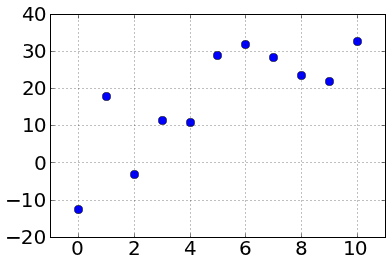
\includegraphics{img/fig1.png}

When we do a linear regression, we fit to a standard ``$y=mx+b$'' form.
For this data, the best fit is
\beqn
y=3.4 x + 0.27,
\eeqn
with a mean squared error of 77.9.  This difference from the line to the data is one measure of how well the line compares to the data - lower values means a better fit, a mean squared error of zero means a {\em perfect} fit.

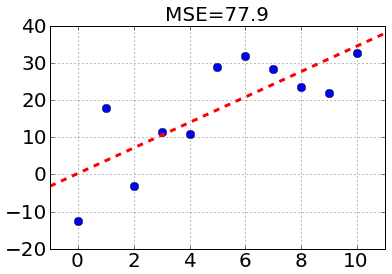
\includegraphics{img/fig2.png}

Overall, not a bad looking fit. However, if we fit to a more complex function, say a 10$^{\rm th}$ polynomial, we can get even better!

\beqn
y&=&-0.0007039 x^{10}  + 0.0363 x^9 - 0.8051 x^8 + 10.04 x^7 - 77.13 x^6 +\\
&& 376.5 x^5- 1159 x^4 + 2152 x^3 - 2163 x^2 + 891.8 x^1 - 12.54
\eeqn

with a Mean Squared Error of {\em zero}.

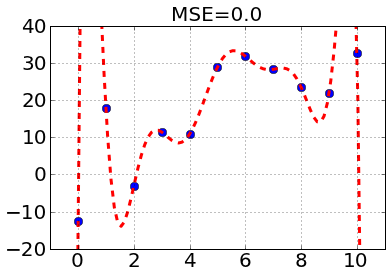
\includegraphics{img/fig4.png}

In the field of statistics, this is referred to as {\em over-fitting}, and is
the result of fitting the variation and not the overall pattern. In other words, it is fitting the
meaningless differences from one point to another by adding a tunable
parameter for each detail in the data. With each new parameter we get a
``better'' fit, by the criterion of mean squared error, but we lose
sight of the meaning. This is the mathematical equivalent of losing
sight of the forest for the trees.

\subsection{Parameters and Ockham's Razor}

When fitting a line, the result is choosing the values of the parameters that have the highest probability given the data.  However, when those parameters can take on any possible value, the overall probability of the model is reduced - this is the probabilistic equivalent of Ockham's Razor which we've seen before in Section~\ref{sec:ockham} on page~\pageref{sec:ockham}.  

We make the problem worse by adding more and more parameters, giving more possible explanatory freedom to our model.  The more freedom we have in choosing the parts of the model, the less explanatory power this model actually has.  One way that statisticians avoid this problem is to fit the model to half of the data, and see how it works on the other half - a process called cross-validation.  A simple model, like a straight line, will do about as well on both.  An overly complex one will do well on the data used to fit it, but will do poorly on new data.

\todo{do an example of this in this case}


\subsection{Back to the Resurrection}\label{back-to-the-resurrection}

If we look at Andy Bannister's very clever solution, we notice something
quite interesting: for every single difference between the Gospel
accounts, he adds a detail not found in the story to explain it. One can
pretty much do this for any two accounts that don't say logically
contradictory things, and can be seen as an example of over-fitting. 

Another way of looking at it is that, if Bannister had constructed his story from, say, two of the Gospel stories and then compared it to the other two he'd have a problem.  Even if he took details from all four accounts, but constructed a story from half of them and then used the other half to confirm it wouldn't work.

As a result, the Easter Challenge, as phrased, is probably not a very good one. One can Rube-Goldberg a story together to fit any amount of details.  Perhaps that is the point, to highlight to what lengths someone has to go to in order to reconcile the four accounts.  However, we think something motivated from cross-validation might be a bit more persuasive.
